
\chapter{Système d'envoi de mail}

Un module du programme permet d'envoyer des mails au créateur de l'ensemble des schémas et au développeurs de l'application. Deux types de mails peuvent être envoyés :\\
\begin{itemize}
\item Une demande d'ajout d'une nouvelle relation. 
\item Un rapport lorsqu'une erreur est survenue dans le logiciel. 
\end{itemize}

\section{Demande d'ajout d'une nouvelle relation}

Dans certains cas, il est possible que l'utilisateur ne trouve pas de relation réelle convenant à la situation qu'il rencontre. L'objectif "Autre" permet de répondre à ce problème. Cependant, si une même relation manque à de nombreuses reprises, il est intéressant d'en informer le créateur de l'ensemble de schémas afin qu'il l'intègre à une futur version.\\

Pour réaliser cette demande, il suffit de cliquer sur l'option "Demande d'ajout de relation" dans le menu "Aide". Une fenêtre s'ouvre alors.\\

L'adresse de réponse permet au destinataire de vous répondre directement.\\

Les deux champs suivants correspondent au sujet et au contenu du mail envoyé.\\


\begin{figure}
\centering
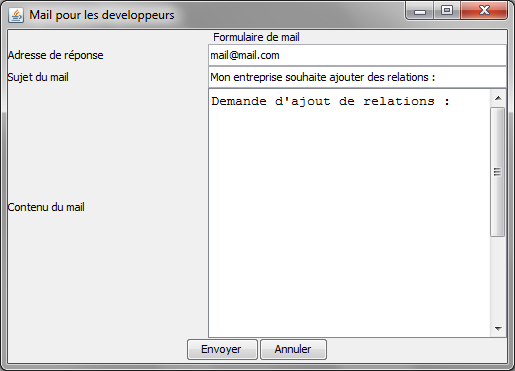
\includegraphics[width=12cm]{images/mail_relation.png}
\caption{La fenêtre du mail de demande d'ajour de relation}
\end{figure}
\section{Envoi d'un rapport d'erreur}
Malgré l'ensemble des tests réalisés sur le logiciel \tria, il est possible qu'il subsiste quelques problèmes. Dans le cas où une erreur est rencontré, le logiciel vous propose automatiquement d'envoyer un mail aux développeurs. Cela leur permet d'identifier l'erreur et de la corriger par la suite.\\

Il est très important de décrire l'action que vous étiez en train de réalisez lorsque l'erreur s'est produite. Cette description est une information souvent indispensable à la résolution du problème. Un texte généré automatiquement à l'intention des développeurs est ajouté à la fin du mail.\\

Une boite de dialogue informe l'utilisateur qu'il est plus prudent de quitter l'application. Si c'est une erreur encore inconnue, il est fortement conseillé de quitter l'application. Dans le cas d'une erreur bénigne, les développeurs informeront l'utilisateur qu'il peut tout de même continuer à travailler (en répondant par mail à l'envoi du rapport d'erreur).\\





